\input{setup/preamble.tex}% package inclusion and set up of the document

%Creates the aau titlepage
\newcommand{\aautitlepage}[3]{%
  {
    %set up various length
    \ifx\titlepageleftcolumnwidth\undefined
      \newlength{\titlepageleftcolumnwidth}
      \newlength{\titlepagerightcolumnwidth}
    \fi
    \setlength{\titlepageleftcolumnwidth}{0.5\textwidth-\tabcolsep}
    \setlength{\titlepagerightcolumnwidth}{\textwidth-2\tabcolsep-\titlepageleftcolumnwidth}
    %create title page
    \thispagestyle{empty}
    \noindent%
    \begin{tabular}{@{}ll@{}}
      \parbox{\titlepageleftcolumnwidth}{
        \iflanguage{danish}{%
          \includegraphics[width=\titlepageleftcolumnwidth]{setup/aau_logo_da.pdf}
        }{%
          \includegraphics[width=\titlepageleftcolumnwidth]{setup/aau_logo_en.pdf}
        }
      } &
      \parbox{\titlepagerightcolumnwidth}{\raggedleft\sf\small
        #2
      }\bigskip\\
       #1 &
      \parbox[t]{\titlepagerightcolumnwidth}{%
      \textbf{Abstract:}\smallskip\par
        \fbox{\parbox{\titlepagerightcolumnwidth-2\fboxsep-2\fboxrule}{%
          #3
        }}
      }\\
    \end{tabular}
    \vfill
    \vspace{-0.5cm}
    \iflanguage{danish}{%
      \noindent{\footnotesize\emph{Rapportens indhold er frit tilgængeligt, men offentliggørelse (med kildeangivelse) må kun ske efter aftale med forfatterne.}}
    }{%
      \noindent{\footnotesize\emph{The content of this report is freely available, but publication (with reference) may only be pursued due to agreement with the author.}}
    }
    \clearpage
  }
}

%Create english project info
\newcommand{\englishprojectinfo}[8]{%
  \parbox[t]{\titlepageleftcolumnwidth}{
    \textbf{Title:}\\ #1\bigskip\par
    \textbf{Theme:}\\ #2\bigskip\par
    \textbf{Project Period:}\\ #3\bigskip\par
    \textbf{Project Group:}\\ #4\bigskip\par
    \textbf{Participant(s):}\\ #5\bigskip\par
    \textbf{Supervisor(s):}\\ #6\bigskip\par
    \textbf{Copies:} #7\bigskip\par
    \textbf{Page Numbers:} Fucking mange!\bigskip\par
    \textbf{Date of Completion:}\\ #8
  }
}

%Create danish project info
\newcommand{\danishprojectinfo}[8]{%
  \parbox[t]{\titlepageleftcolumnwidth}{
    \textbf{Title:}\\ #1\bigskip\par
    \textbf{Theme:}\\ #2\bigskip\par
    \textbf{Project Period:}\\ #3\bigskip\par
    \textbf{Project Group:}\\ #4\bigskip\par
    \textbf{Participants:}\\ #5\bigskip\par
    \textbf{Supervisor:}\\ #6\bigskip\par
    \textbf{Copies:} #7\bigskip\par
    \textbf{Page Numbers:} ??
    \bigskip\par
    \textbf{Date of Completion:}\\ #8
  }
}

%Nice-looking reference to other chapters
\newcommand{\chapref}[1]{Chapter \ref{#1}: \nameref{#1}}
\newcommand{\secref}[1]{Section \ref{#1}: \nameref{#1}}
\newcommand{\figref}[1]{\emph{Figure: \ref{#1}}}
\newcommand{\appref}[1]{\emph{Appendix \ref{#1}}}
\newcommand{\tabref}[1]{\emph{Table: \ref{#1}}}
\newcommand{\coderef}[1]{\emph{Listings: \ref{#1}}}
\renewcommand{\eqref}[1]{\emph{Equation: (\ref{#1})}}

\newcommand{\iic}[0]{I²C }

%%%%%%%%%%%%%%%%%%%%%%%%%%%%%%%%%%%%%%%%%%%%%%%%
% An example environment
%%%%%%%%%%%%%%%%%%%%%%%%%%%%%%%%%%%%%%%%%%%%%%%%
\theoremheaderfont{\normalfont\bfseries}
\theorembodyfont{\normalfont}
\theoremstyle{break}
\def\theoremframecommand{{\color{aaublue!50}\vrule width 5pt \hspace{5pt}}}
\newshadedtheorem{exa}{Example}[chapter]
\newenvironment{example}[1]{%
		\begin{exa}[#1]
}{%
		\end{exa}
}

\makeatletter
\newcommand{\ChapterOutsidePart}{%
   \def\toclevel@chapter{-1}\def\toclevel@section{0}\def\toclevel@subsection{1}}
\newcommand{\ChapterInsidePart}{%
   \def\toclevel@chapter{0}\def\toclevel@section{1}\def\toclevel@subsection{2}}
\makeatother

\usepackage{bookmark}

\usepackage{mathtools}
\DeclarePairedDelimiter{\ceil}{\lceil}{\rceil}








%Figure references:
%\newcommand{\figref}[1]{\textbf{figure \ref{#1}}}

%Figure references after full stop/period:
\newcommand{\Figref}[1]{\textbf{Figure \ref{#1}}}

%Table references:
\newcommand{\tableref}[1]{\textbf{table \ref{#1}}}

%Table references after full stop/period:
\newcommand{\Tableref}[1]{\textbf{Table \ref{#1}}}

%Units:
\newcommand{\unit}[1]{&& \left[\si{#1}\right]}

%Text:
\newcommand{\tx}[1]{\text{#1}}

%Equation references:
%1 equation:
\renewcommand{\eqref}[1]{\textbf{equation (\ref{#1})}}
%2 equations:
\newcommand{\eqrefTwo}[2]{\textbf{equation (\ref{#1})} and \textbf{(\ref{#2})}}
%3 equations:
\newcommand{\eqrefThree}[3]{\textbf{equation (\ref{#1})}, \textbf{(\ref{#2})} and \textbf{(\ref{#3})}}
%4 equations:
\newcommand{\eqrefFour}[4]{\textbf{equation (\ref{#1})}, \textbf{(\ref{#2})}, \textbf{(\ref{#3})} and \textbf{(\ref{#4})}}
%5 equations:
\newcommand{\eqrefFive}[5]{\textbf{equation (\ref{#1})}, \textbf{(\ref{#2})}, \textbf{(\ref{#3})}, \textbf{(\ref{#4})} and \textbf{(\ref{#5})}}
%6 equations:
\newcommand{\eqrefSix}[6]{\textbf{equation (\ref{#1})}, \textbf{(\ref{#2})}, \textbf{(\ref{#3})}, \textbf{(\ref{#4})}, \textbf{(\ref{#5})} and \textbf{(\ref{#6})}}
%7 equations:
\newcommand{\eqrefSeven}[7]{\textbf{equation (\ref{#1})}, \textbf{(\ref{#2})}, \textbf{(\ref{#3})}, \textbf{(\ref{#4})}, \textbf{(\ref{#5})}, \textbf{(\ref{#6})} and \textbf{(\ref{#7})}}

%Equation references after full stop/period:
%1 equation:
\newcommand{\Eqref}[1]{\textbf{Equation (\ref{#1})}}
%2 equations:
\newcommand{\EqrefTwo}[2]{\textbf{Equation (\ref{#1})} and \textbf{(\ref{#2})}}
%3 equations:
\newcommand{\EqrefThree}[3]{\textbf{Equation (\ref{#1})}, \textbf{(\ref{#2})} and \textbf{(\ref{#3})}}
%4 equations:
\newcommand{\EqrefFour}[4]{\textbf{Equation (\ref{#1})}, \textbf{(\ref{#2})}, \textbf{(\ref{#3})} and \textbf{(\ref{#4})}}
%5 equations:
\newcommand{\EqrefFive}[5]{\textbf{Equation (\ref{#1})}, \textbf{(\ref{#2})}, \textbf{(\ref{#3})}, \textbf{(\ref{#4})} and \textbf{(\ref{#5})}}
%5 equations:
\newcommand{\EqrefSix}[6]{\textbf{Equation (\ref{#1})}, \textbf{(\ref{#2})}, \textbf{(\ref{#3})}, \textbf{(\ref{#4})}, \textbf{(\ref{#5})} and \textbf{(\ref{#6})}}
%5 equations:
\newcommand{\EqrefSeven}[7]{\textbf{Equation (\ref{#1})}, \textbf{(\ref{#2})}, \textbf{(\ref{#3})}, \textbf{(\ref{#4})}, \textbf{(\ref{#5})}, \textbf{(\ref{#6})} and \textbf{(\ref{#7})}}% my new macros

\usepackage{lastpage}
\usepackage{epstopdf}

\setlength{\headheight}{21pt}

\hfuzz=\maxdimen
\tolerance=10000
\hbadness=10000

\usepackage{siunitx}

\graphicspath{{./figures/}}

\begin{document}
%% prereport %%
\setlength\cftaftertoctitleskip{2pt}
\setlength\cftafterloftitleskip{6pt}
\setlength\cftafterlottitleskip{6pt}

\selectlanguage{english}
\title{AAUSAT 6}

\pagestyle{empty} %disable headers and footers
\pagenumbering{roman} %use roman page numbering in the frontmatter I II...
\fancyfoot[RE,LO]{15gr510} %page number on all pages
\fancyfoot[LE,RO]{\thepage}
\fancyhead[LE,LO,RE,RO]{}

%% indledende formalia %%
%\includepdf[pages={1}]{forside2.pdf}
%\pdfbookmark[0]{Frontpage}{label:forside}%
\begin{titlepage}
  \addtolength{\hoffset}{0.5\evensidemargin-0.5\oddsidemargin} %set equal margins on the frontpage - remove this line if you want default margins
  \noindent%
  \begin{tabular}{@{}p{\textwidth}@{}}
    \toprule[2pt]
    \midrule
    \vspace{0.2cm}
    \begin{center}
    \Huge{\textbf{
      AAUSAT6 Camera solution % insert your title here
    }}
    \end{center}
    \begin{center}
      \Large{
      an image capturing unit for use in a cubesat
      }
    \end{center}
    \vspace{0.2cm}\\
    \midrule
    \toprule[2pt]
  \end{tabular}
   \vspace{0.55 cm}
  \begin{figure}[!ht]
\centering
\includegraphics[width=\textwidth]{Kerbal.png}
\label{fig:forside}
\end{figure}
  \vspace{-0.35 cm}
  \begin{center}
    {\large
      P4 project report %Insert document type (e.g., Project Report)
    }\\
    \vspace{0.2cm}
    {\Large
      Group 413%Insert your group name or real names here
    }
  \end{center}
  \begin{center}
  Aalborg University\\
  Electronic Engineering \& IT\\
  Frederiks Bajersvej 7\\
  DK-9000 Aalborg
  \end{center}
\end{titlepage}

\clearpage
\pagestyle{fancy}
\include{formalia/kolofon}
\input{formalia/titlesheet.tex}

\pdfbookmark[0]{Indholdsfortegnelse}{label:Indhold}
\tableofcontents

%\printglossary[title=List of Terms,toctitle=Terms and abbreviations,type=\acronymtype]

%\glsaddall
%\printglossary
%\printglossary[type=\acronymtype]

%\listoftodos

% Preface %
\chapter*{Preface}
The project is to design a autonomous vehicle able to 

Text by:\\
%
\begin{table}[H]
	\centering
		\begin{tabular}{c c c}
			\underline{\phantom{JAERJAERJAERJAERGO}} & \phantom{cookies} & \underline{\phantom{JAERJAERJAERJAERGO}} \\
			Amalie V. Petersen			& \phantom{cookies} & Julien Br\'ehin		\\
			&&\\
			&&\\
			\underline{\phantom{JAERJAERJAERJAERGO}} & \phantom{cookies} & \underline{\phantom{JAERJAERJAERJAERGO}} \\
			Mads Gotthardsen			& \phantom{cookies} & Niels Skov Vestergaard		\\
			&&\\
			&&\\
	    \underline{\phantom{JAERJAERJAERJAERGO}} & \phantom{cookies} & \underline{\phantom{JAERJAERJAERJAERGO}} \\
			Romaric Destremau 					& \phantom{cookies} & Thomas Rasmussen 			\\			
		\end{tabular}
\end{table}

\cleardoublepage

%% problemanalysen %%
\pagenumbering{arabic} %use arabic page numbering in the mainmatter
\fancyfoot[RO,LE]{\thepage \text{ of} \pageref{LastPage}}
\fancyfoot[LO,RE]{15gr412}
\fancyhead[RE,LO]{}
\fancyhead[RE,LO]{\color{aaublue}\small\nouppercase\leftmark} %even page - chapter title

\fancyhead[RO,LE]{
\includegraphics[height=16pt]{logo_only.pdf}}


\pagestyle{fancy}

% \include{kapitler/indledning}


% %% Part 1 %%

\part{Preanalysis}

\chapter{Introduction}
More and more robots appear in everyday life. Automatic vacuum cleaners and floor washers are getting widespread, as the technology is becoming cheaper and better. The vacuum cleaners have matured to a level, where they are been considered for saving man-hours in the elderly care sector.\\\\
Outside the walls of our homes lays the next weekly hurdle: mowing the lawn. A known way to handle this, is to pay the neighbour's teenager to do it. Unfortunately they grow up and move out, leaving the lawns in the residential neighbourhoods behind.\\\\
Luckily engineers have stepped in, and provided a more long-term solution: robotic lawn mowers.
\chapter{Design Consideration}
\vspace{-5 mm}
In this chapter the system is designed with a top-down approach. First a use-case of the functionalities in the system is described, in order to give an overall view of what the system must be able to do. Hereafter, constraints set by time limitations as well as a focus on the main scope of the project, in regards to the prototype, is considered. Based on the use-case description and the prototype constraints the requirements for the systems prototype are listed.
\vspace{-4 mm}
\section{Use-case design}
To give an overall view of what the system should be able to do, a UML use-case diagram is used to consider and describe the main functionalities and operators in the system, see \figref{fig:usecase}.
\vspace{-3 mm}
 \begin{figure}[H]
	\centering
	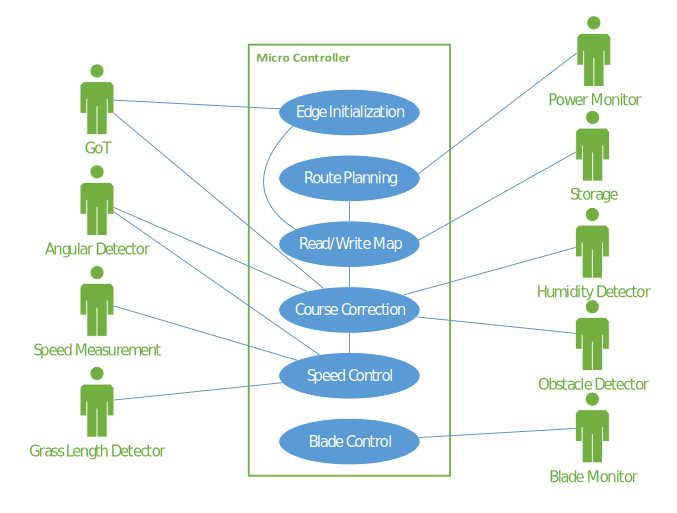
\includegraphics[scale=0.8]{figures/P5UseCase.pdf}
	\caption{Use-Case Diagram}
	\label{fig:usecase}
\end{figure}\vspace{-5mm}

\noindent
The main purpose of the system is to automatically navigate in a specific area which is confined by the \textit{edge initialization} functionality. This functionality handles the marking of the areas edges. The functionality is only used in the initialization process of the system. The concept is to only use the functionality after the GoT system has been positioned in the area. The consumer then takes the system around the edges of the grass, while the GoT system tracks its positions. It is therefore only necessary to reinitialize the system, if the GoT satellites has been moved. While the edge is being tracked, the \textit{edge initialization} uses the \textit{read/write map} functionality to store the information collected, in storage. \\\\ 
\noindent
The route in which the lawn mower is to navigate, in the specified area, is provided by the functionality \textit{route planning}. \textit{Route planning} uses the information, about the specific area, which is collected from the storage, to plan the most optimal route. Furthermore the \textit{route planning} needs information about the systems power level to insure the functionality is considering if the system needs charging and therefore have to return to the charging station at some point on the route.\\\\
\noindent
The \textit{read/write map} functionality as described earlier, handles the communication with storage. Hence it stores information, received from the \textit{edge initialization} and collects information from storage when the functionality \textit{route planning} needs it. \\\\
\noindent
To insure the system is moving with a desired speed (in a straight line and in a turn) or a speed which is fitted to the height of the grass, detected with the \textit{grass length detector}, a \textit{speed control} functionality is necessary in the system to control the motors. To insure the \textit{speed control} can deliver the desired speed an \textit{angular sensor} is utilized. \\\\
\noindent
The last functionality, \textit{course correction} is used when the system strays of the path calculated by \textit{route planning} or if the path gets blocked.
The obstacle which is blocking the route is detected by the sensor \textit{obstacle detector}. Furthermore the GoT system and the \textit{angular detector} will detect if the system is not on the desired path, or if the system starts to slip. Also, if it starts to rain, which is detected by the \textit{rain detector}, the system has to return to the charging station.
Finally, the \textit{course correction} sends the calculated data to the functionality \textit{speed control}. \\\\
\noindent
The overall functionalities of what the system must be able to do has been described. Now the different constraints on the system will be considered and the project prototype should be established.
\section{Prototype Constraints}
Before the prototype can be established, some considerations have to be made in respect to the time limitations and the main scope of this semester. The aim of the project is to create a functional automated proof of concept lawn mower. The following section includes a brief description of the technology on which the prototype is constructed, along with argumentation for eliminated functionalities.

\subsection{Technology Base}
The technology which has been provided for the prototype is a tracked vehicle, seen on \figref{TrackedVehicle}. The vehicle comes with a brushed DC motor which provides power for rotation of the wheels connected to the belts. Furthermore a servo motor is used to control the ratio of the differential steering, by utilize breaks connected to the wheels. The tracked vehicle includes two hall sensors, one by each belt, which keeps track of the speed, of the belts, by measuring pulses from magnets mounted on the front wheels. The testing will take place in Aalborg University Vicon Room, where the GoT system is installed and calibrated with the appurtenant transmitter, which is mounted on the tracked vehicle during test.

\begin{figure}[H]
	\centering
	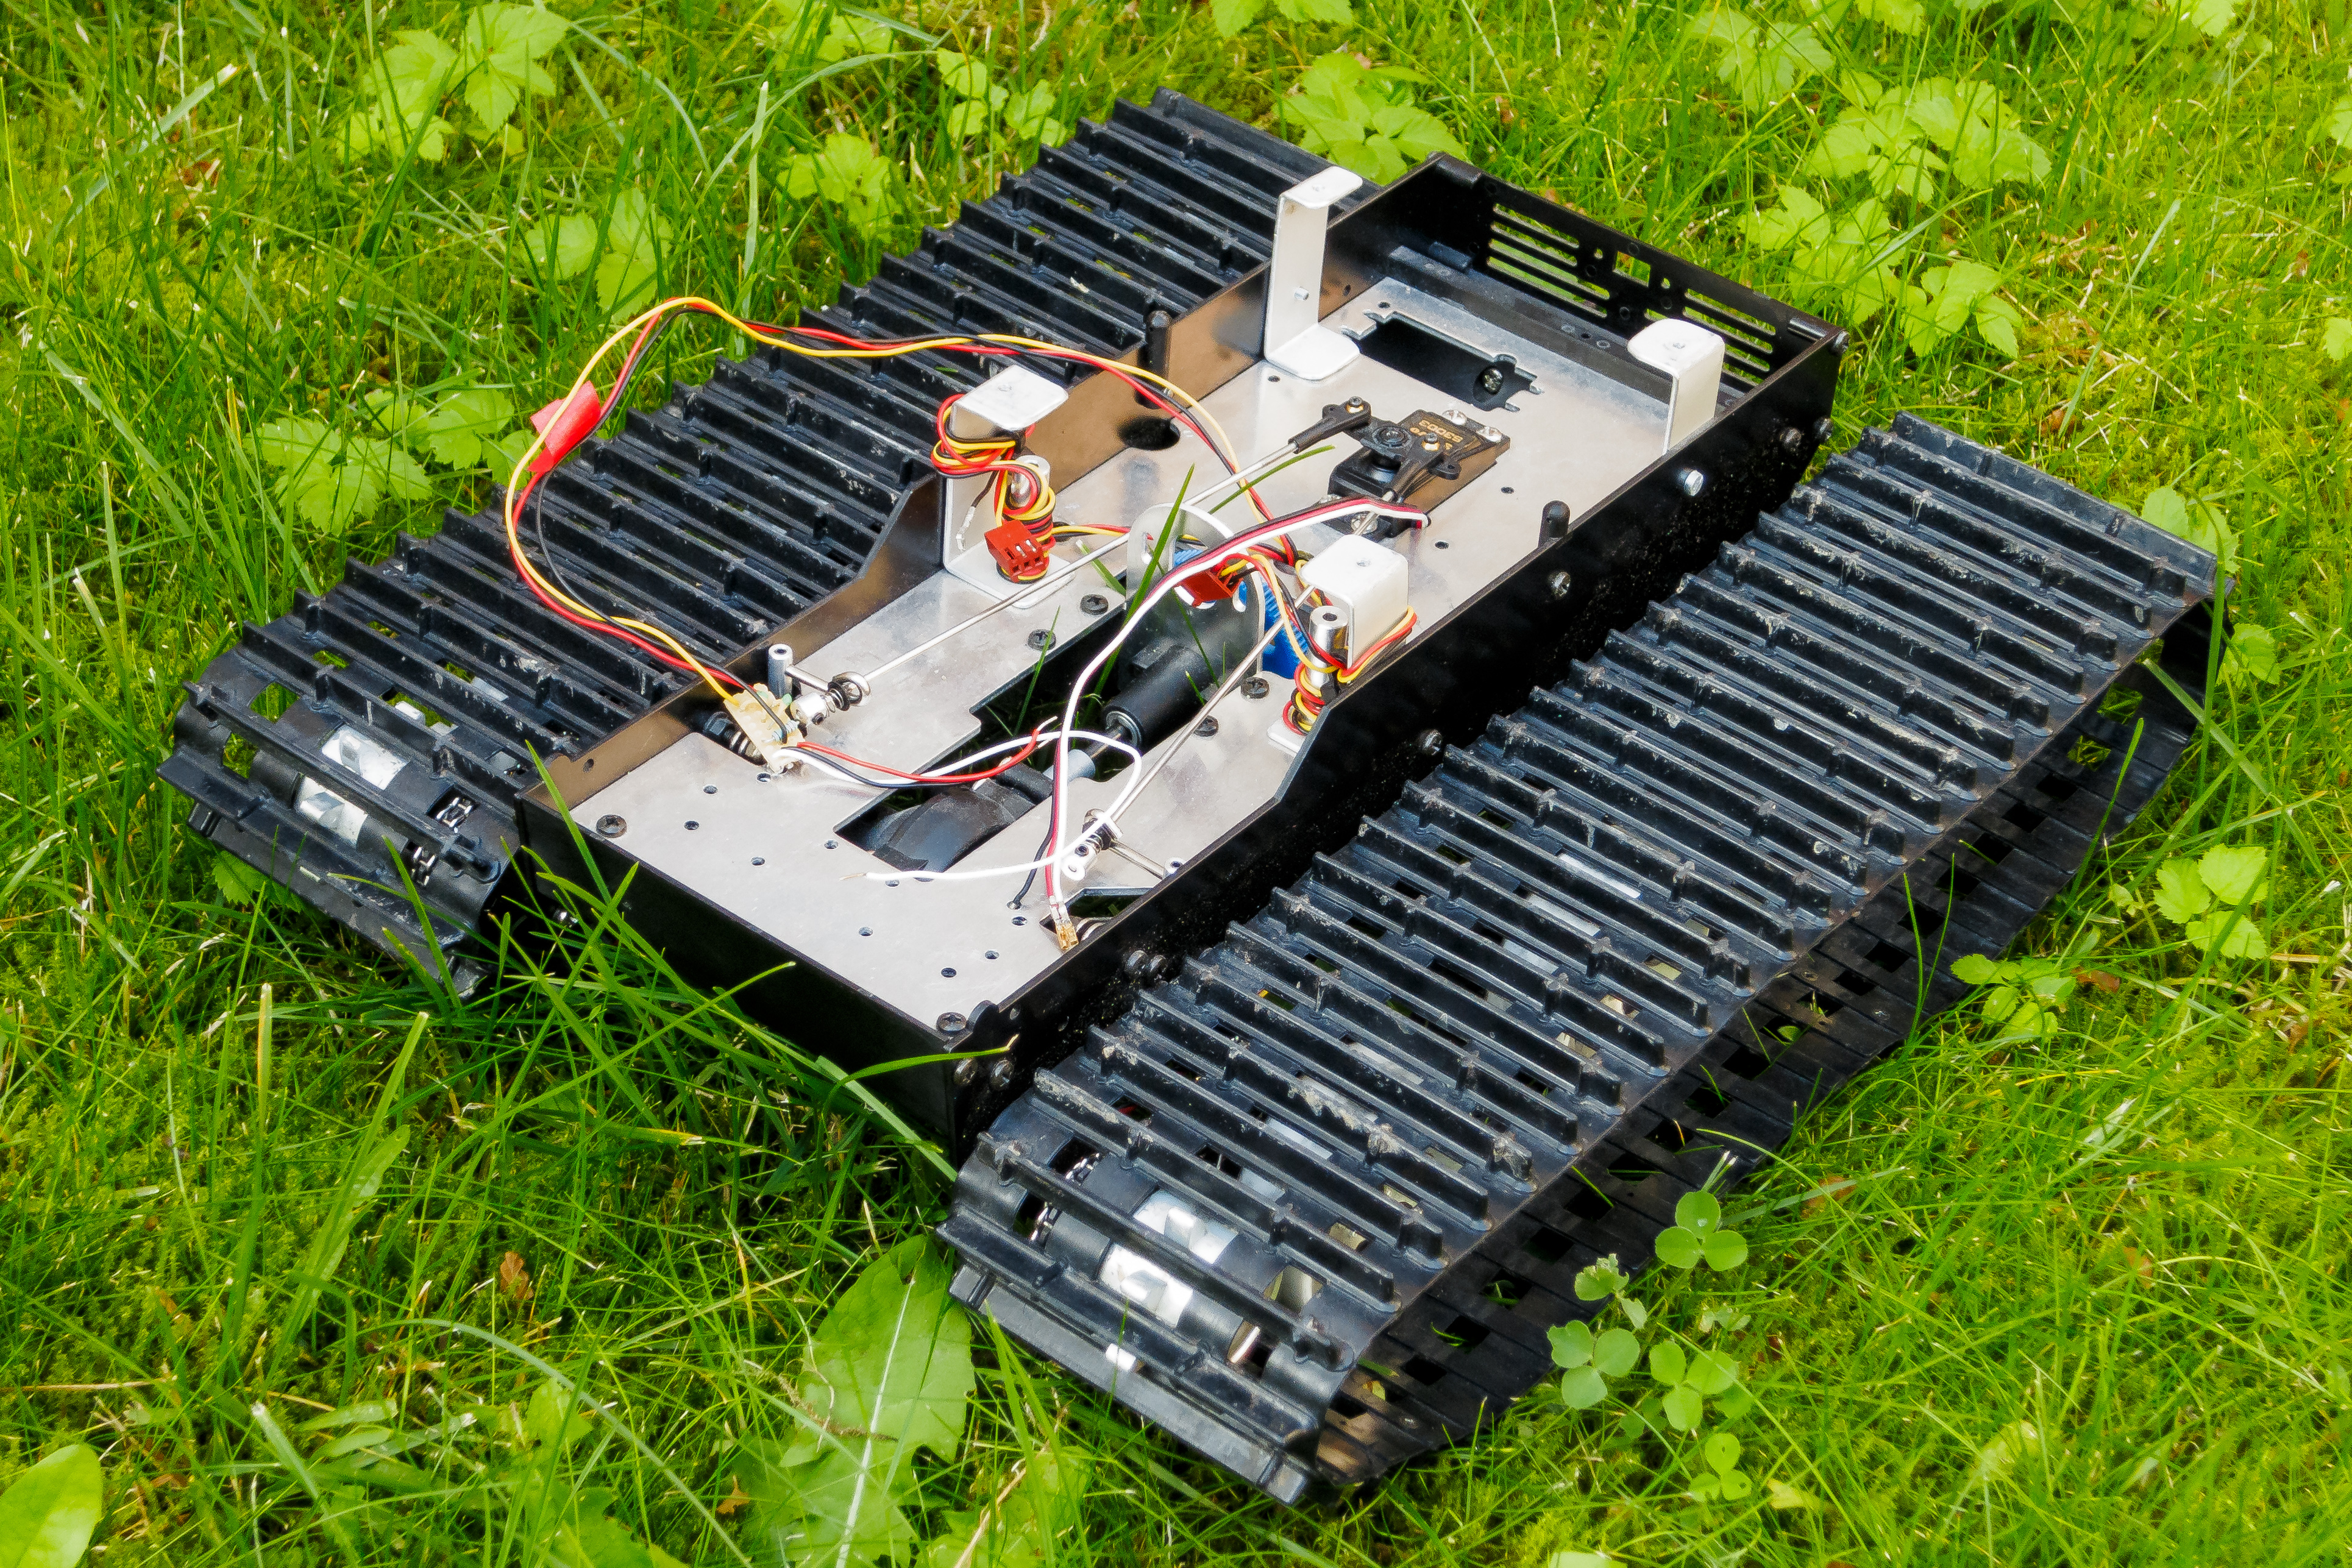
\includegraphics[scale=0.8]{figures/BeltVehicle.jpg}
	\caption{The provided track vehicle}
	\label{TrackedVehicle}
\end{figure}

\todo{datasheet of the vehicle}

\subsection{Grass Length Detection}
Detection of the grass length to control the speed of the lawn mower thus ensuring an evenly cut lawn, is a submodule which can be added at any time. Since it is not fatal for a working system and might even be unnecessary depending on time between each mowing of the lawn, it is decided to exclude this functionality from the initial design.

\subsection{Humidity Sensor}
As the lawn mower is supposed to work outside, it is important to consider that the grass could be humid. Since it is difficult to cut humid grass, a humidity sensor could be used to warn the system of the humidity. Thus the system could go back to the charging station. However, the prototype will only be tested indoor, so this type of sensor will not be necessary in a prototype design.

\subsection{Obstacle Avoidance}
The lawn movers path might not always be clear, e.g. garden tools, tables or moving objects could be in the way. The vehicle should be aware of what is in front of it at any time, to correct its path and get around the obstacle if necessary. To avoid this the sensor could be a pushing button to detect a solid object or an ultrasound detector if the object is fragile.
As the aim of the project is to control the path of the vehicle by using angular positioning sensors, a proximity sensor will not be included. Static objects could be registered on the map to avoid these issues.\\\\
Furthermore the edge mapping functionality will not be included in the project which instead will focus on a quadratic map predefined in the test room.

\subsection{Power Monitoring}
Power monitoring could be implemented by measuring the voltage across the batteries, to ensure that the lawn mower is not running out of power, and to ensure the vehicles calculated route passes the charging station before the power runs too low.
This and the charging station will not be in the prototype, since it is beyond the scope of the project this semester and is not crucial for a working prototype.

\section{Prototype, Interfaces and Submodules} \label{Finalprototype}
%The overall functionalities for the project have been limited, due to time limitations and to focus on the scope of the project. In this project a prototype will therefore be made to show the main functionalities necessary to make an automated vehicle containing principles for lawn mowing.
%In short, the final prototype includes a regulator, which will make it possible to follow a path from A to B. It is able to continue if the wireless connection is lost between the prototype and the GoT system for some duration. Furthermore it is able to plan a route within a given area and store these calculated data points locally, on the vehicle. The rough outline of the design is shown in \figref{fig:systemOverview1} to give an idea of the final prototype setup.

%\begin{figure}[H]
%	\centering
%	\includegraphics[scale=.9]{figures/systemOverview1}
%	\caption{Overview of the system prototype}
%	\label{fig:systemOverview1}
%\end{figure}

%The GoT system provides the vehicle with coordinates, which is utilized in course correction in combination with the map supplied from storage, to follow the route. In course correction lies also control between coordinates given by the GoT system and the storage, this is regulated through use of angular position and movement supplied by the angular sensors. The speed control gets an input from the course correction, the speed given is then held through regulation again using input from angular sensors, in this case specifically acceleration.


%Previously the rough prototype design is presented. To provide a more broad overview of the system, an exploded view of functionalities, their submodules and interfaces is presented in \figref{fig:systemOverview2}.

The overall functionalities for the project have been constrained from the Use-Case \secref{sec:UseCase}, due to time limitations and to focus on the main scope of the semester. A prototype is therefore made to illustrate the main functionalities necessary to make an automated vehicle, containing principles for lawn mowing.

The final prototype includes a regulator, which will make it possible to follow a path from A to B. It is able to continue if the wireless connection is lost between the prototype and the GoT system for some duration. The outline of the design is shown in \figref{fig:systemOverview2} to give an idea of the final prototype setup. In this section, the different functional blocks are put forth along with the interfaces describing the interaction between them.

\begin{figure}[H]
	\centering
	\includegraphics[scale=.9]{figures/systemOverview2}
	\caption{Overview of the software and electronic parts of the system prototype, where the gray modules are hardware and the white are software. The dotted lines are wireless signals while the others are wire signals}
	\label{fig:systemOverview2}
\end{figure}

\subsection{Modules}
In the following all the modules from the system prototype which needs further explanation are described to obtain a basic understanding of the prototype.

%\subsubsection{GoT System}
%%The GoT satellites is placed in the area in which the vehicle needs to operate. These satellites receives information from the vehicle. The time which the vehicles transmitter sends out bursts is received by the GoT master. Furthermore the time which the satellites receives the information send from the vehicles transmitter is transmitted to the GoT master. The GoT master then relays the information received from the vehicle directly to the 
%
%The \textit{GoT Transmitter} placed on the vehicle transmits a signal containing the time at which it send the ultra sound signal to the \textit{GoT Satellites} to the \textit{GoT Master}. The satellites transmit the signal recieved to the master as soon as they recieve it. The master then relays those informations to the \textit{GoT on Computer} that will calculate the position of the car.

\textbf{Computer and Position Decoder:}
The computer handles the calculation of the current position of the vehicle \appref{GoTDescription}. If a packet is disturbed or sent incorrectly it should be possible to detect it, so invalid data is not used by the prototype. It may occur that the coordinates which are sent from the GoT system is out of sensible range, e.g the coordinate transmitted jumps from one location to a location which is unrealistic, for the vehicle to reach in the amount of time between received coordinates. In this event the out of range coordinate should also be disregarded. The computer must compile a package containg the coordinates. The position decoder must be able to decode the send package.

\textbf{Course Correction:}
This module receives the vehicles position from the GoT and the next destination on the path, which is located in the storage. These informations constitutes a path segment on which it is the course correction's task to stay. To accomplish this it receives the angle and the speed of the vehicle, and uses this information to correct its course along the current path segment.

\textbf{Read/Write Map:}
This module handles the writing of coordinates to the nonvolatile storage device, as well as the reading of next desired destination from the stored map.

\textbf{Speed Control:}
This module retrieves the speed of the vehicle from the Get Speed module. This is used, through control, to obtain a steady speed. Furthermore it handles any request of change in speed delivered by the course correction.

%\subsubsection{Edge Map}
%The first time the user will initialise the lawn mower, an \textit{Edge Map} will be created thanks to the GoT system. This edge map will determine the areas that the car is allowed to go or not, in regards of specifications or objects on the lawn.  

%\subsubsection{Route Planning}
%The Route Planning module calculates a route from the points gathered from the Edge Map. The route will be in straight lanes, as in the Bosch Logicut system \secref{roboMowers}, to guarantee that the whole lawn is cut.

%\subsubsection{Angular Sensors}
%The angular position is measured thanks to the \textit{Angular Sensors}, that will send data to the submodule \textit{Get Angle}, in charge to send the angle to the Speed Control and to the Course Correction submodule.

\subsection{Interfaces}
%- To Tom and Rasmus \newline
%In the subsection an explanation of the different interfaces between the modules is made. We have thought about making it like a high layer interface, where we only explain what we need the different modules to give each other. Like one module needs to get the map edge, i.e. coordinates, but since it is this early in the report and it would be more overview by writing map edge rather than coordinates. But as you can see in \figref{fig:systemOverview2} the layers of information are different, one is raw angle data and another time send. Is this okay or should we change something else?
%\indent
%The interfaces of the system is very important when designing each of the adjacent submodules. The existing interfaces as well as the ones presumed are also important in the process of analyzing the system capabilities width focus on requirements of the prototype. Width that in mind follows a brief review of the interfaces between each submodule.
In this section a high layer interface between the modules will be presented. This provides information for designing each of the adjacent submodules individually.

\textbf{8 - Package Containing Position:}
The data communicated from the GoT system to the vehicle contains the last recorded position of the vehicle. This position is presented in the form of an x- and a y-coordinate, which must be included in the data package. Additionally each package must contain decode information for the receiver, including how to separate each package along with error handling.

\textbf{7 \& 4 - Angle/Servo Control Signal \& PWM Signal:}
Course correction will ask the vehicle to turn or make small adjustments of the angle. This angle is realized through the servo motor which breaks on either belt aproprite to the required angle. For the servo to understand the angle the servo driver must translate it into a PWM signal, which makes the servo turn to a specific position for each pulse width.

\textbf{2 \& 1 - Angle \& Raw Angle Data:}

\textbf{6, 5 \& 4 - Desired Speed, Motor Control Signal \& PWM Signal:}

\textbf{11 \& 3 - Hall Sensor Pulses \& Belt Speed:}

\textbf{13 - Route Coordinates:}






%Route Planning, Storage and Read/Write Map Interfaces:
%The Edge Map submodule sends the Map edge to Route Planning, that will send a Route to Read/Write Map. The Route to follow will then be transmited to the Course Correction submodule for a path correction, and to the Storage for saving.

%\textbf{Speed Control Interfaces:}
%The Hall Sensors send Hall sensor pulses to the submodule Get Speed, that will process it to transmit the Belt speed to the Speed Control. A PWM signal containing the new wanted speed will then be sent to the Motor Driver, wich will convert it to the final Motor control signal and sent it to the Drive Motor.
%
%\textbf{Angular Sensors Interfaces:}
%The Angular Sensors will send a Raw angle data to the submodule  Get Angles, that will process it and send the Processed angle data to Course Correction.
%
%\textbf{Course Correction Interfaces:}
%The Course Correction submodule receives the Position and Time from the Wireless Module, the Route to follow from Read/Write Map, and the Processed angle data from Get Angles. With all those information, a decision will be sent to the Speed Control through the Desired speed, and to the Servo Motor with an Angle/servo control signal.

Now that the vehicle had been described and the prototype defined, the modeling of the vehicle can be made.


%---------------------------------------------------------------------------------------------------------------------------\\
%REWRITE THIS SCRAMBLED VERSION OF THE ABOVE TWO SUBSECTIONS \todo{rewrite in the above section and delete these subsections}\\
%---------------------------------------------------------------------------------------------------------------------------
%
%\subsubsection{GoT Satellites, Master and GoT Ultra Sound \& Radio Link}
%\indent
%A number of GoT Satellites are placed in the corners of the area in which the vehicle is to operate. These Satellites receive ultra sound signal from the GoT device placed on the vehicle. The time in which each ultrasound signal is received is passed through a wireless connection from the satellites to the GoT master. The GoT master then pairs this information with the time the ultra sound signal was send from the vehicle which it receives via radio link from the GoT device on the vehicle. After collecting the information, the GoT master sends a calculated position and along with a time stamp to the computer handling GoT.
%
%\subsubsection{Wireless Modules}
%\indent
%%The wireless modules serves the purpose of transmitting the calculated coordinates from the GoT system to the vehicle.
%
%\subsubsection{Edge Map, Route Planning, Read/Write Map and Storage}
%\indent
%%The route planning functionality receives the hard coded edge positions from edge map. Using this information the route is then planned and saved in the storage through the read/write map functionality.
%
%\subsubsection{Gyro, Accelerometer, Magnetometer, Speed Control and Course Correction}
%\indent
%%Gyro along with magnetometer is used for angular position of the vehicle. This is passed to the course correction through the get angle functionality. Here it is used as to correct the orientation of the vehicle on its path. The accelerometer also channels through the get angle functionality. The angular acceleration is then used for correction of the speed.
%
%\subsubsection{Hall Sensor}
%\indent
%%The speed control also receives input from the hall sensors through the get speed functionality, where the inputs from the hall sensors are translated to speed of the vehicle's belts. This information is then used in speed control to regulate the speed.
%
%\subsubsection{Servo Motor}
%\indent
%%The servo motor receives an angle/servo control signal from course correction. This angle equals a given amount of breaking on either of the two belts, which then through the differential gearing translate into steering and thus correction of the course of the vehicle.
%
%\subsubsection{Motor Driver and Drive Motor}
%\indent
%%The drive motor takes a motor control signal from the motor driver provided by the speed control. The control signal from speed control is a PWM signal.

% %% Part 2 %%

\part{Design \& implementation}

% %% Part 3 %%

\part{Test \& conclusion}

%% literaturliste og bilag %%
\bookmarksetup{startatroot}% this is it
\addtocontents{toc}{\bigskip}% perhaps as well
%\bibliography{setup/mybib}
%\label{bib:mybiblio}
 
 \newpage
 \fancyhead[RO]{\color{aaublue}\small Appendix \nouppercase\rightmark} %even page - chapter title
 \fancyhead[LE]{\color{aaublue}\small Appendix \nouppercase\rightmark} %uneven page - sectionhttps://88df6ea0630aed8027ff-0caf779119a6537399728d4d80523795.ssl.cf5.rackcdn.com/tcgyzshtzfpq/page/7cd587cdbc0ae962c2755c91cf17670aac438f1c.jpeg title
\fancyhead[RE,LO]{}
 \titleformat{\section}[hang]{\Large\bfseries}{\thesection\hsp\textcolor{aaublue}{|}\hsp}{0pt}{\Large\bfseries}

 \renewcommand{\thesection}{\Alph{section}}
 \setcounter{section}{0}

% %% Appendix %% 
 
 \chapter*{Appendix}
 \addcontentsline{toc}{chapter}{Appendix}
	%\section{Figure Sample}

\begin{figure}[H]
	\caption{CAPTION\fxnote{Remember source}}
	\label{LABEL}
	\centering
	\includegraphics[scale=.6]{figures/filename}
	\flushleft
	\textit{SOURCE}
\end{figure}

%--------- NOTES ------------------------------------------------------
%Fxnotes wont compile properly inside the figure, only in the caption.
%Filetype ([...]{figures/filename.jpg}) can be specified but isn't needed.

\figref{LABEL} \Figref{LABEL}

%Do not use \vspace{length} or \hspace{length} or \noindent etc unless exceedingly necessary - LaTeX is a markup language, let it do its job.
\vspace{.5cm}
\noindent
%--------- BIBLIOGRAPHY REF EKSAMPLE -----------------------------------
This reference only represents this line since it is before the punctuation mark\cite{YDing}. This next reference however represents the entire section. That is all of the preceding sentences in the entire section. This is due to the fact that it is now after the punctuation mark in the end of the section (this is not used in the middle of a section!).\cite{YDing}
%>>>>>>>>>>>>>>>PLEASE ALSO READ THE NOTE IN bibliography/bibliography.bib<<<<<<<<<<<<<<<<<<
\pagebreak
	%\input{Appendix/aTestTemplate.tex}
	%\input{Appendix/bTableSample.tex}
	%\section{Equation Sample}

Ohms Law:
\begin{flalign}
  U &= I \times R \unit{\volt}
  \label{eq1}
\end{flalign}
%
Some explanation:
\begin{flalign}
  [Equation] &= [Number] \unit{Unit}
  \label{eq2}
\end{flalign}
%
Some explanation:
\begin{flalign}
  [Equation] &= [Number] \unit{Unit}
  \label{eq3}
\end{flalign}
%
Some explanation:
\begin{flalign}
  [Equation] &= [Number] \unit{Unit}
  \label{eq4}
\end{flalign}
%
Some explanation:
\begin{flalign}
  [Short Equation] &= [Number] \unit{Unit}
  \label{eq5}\\ %<-------------------------------------------------| Remember linebreak AFTER
  [Somewhat Longer Equation] &= [Number] \unit{Unit} %             | label when writing multiple
  \label{eq6}\\ %<-------------------------------------------------| equations.
  [Somewhat Quite a Lot Longer Equation] &= [Number] \unit{Unit}
  \label{eq7}
\end{flalign}
%
%
\eqref{eq1}\\
%
\eqrefTwo{eq1}{eq2}\\
%
\eqrefThree{eq1}{eq2}{eq3}\\
%
\eqrefFour{eq1}{eq2}{eq3}{eq4}\\
%
\eqrefFive{eq1}{eq2}{eq3}{eq4}{eq5}\\
%
\eqrefSix{eq1}{eq2}{eq3}{eq4}{eq5}{eq6}\\
%
\eqrefSeven{eq1}{eq2}{eq3}{eq4}{eq5}{eq6}{eq7}\\
%
\Eqref{eq1}\\
%
\EqrefTwo{eq1}{eq2}\\
%
\EqrefThree{eq1}{eq2}{eq3}\\
%
\EqrefFour{eq1}{eq2}{eq3}{eq4}\\
%
\EqrefFive{eq1}{eq2}{eq3}{eq4}{eq5}\\
%
\EqrefSix{eq1}{eq2}{eq3}{eq4}{eq5}{eq6}\\
%
\EqrefSeven{eq1}{eq2}{eq3}{eq4}{eq5}{eq6}{eq7}
%
\pagebreak
	\section{The Games on Track GT-position system}
\label{GoTDescription}
The Games on Track GT-Position system, shortened GoT, is a position system which uses radio-waves and ultrasound to locate the object. The system is build up by three types of hardware components: the transmitter, the satellites and the master, see \figref{GoTSystem}. The transmitter and the satellites send the information in all directions, with a 360 degree signal.\\
The GoT System does not work if the transmitter is not close enough from the satellites or if there is some interference by another signal or by an object between them and therefore can not communicate with the satellites.

\begin{figure}[H]
	\centering
	\includegraphics[scale=0.6]{figures/GoT_description.pdf}
	\caption{Overview of the GoT system}
	\label{GoTSystem}
\end{figure}

\subsubsection{Transmitter}
The transmitter component is placed on the object which needs to be located. The transmitter sends an ultrasound burst out containing his id that the satellites are intended to receive. The time at which each ultrasound bursts are sent from the transmitter to the satellites is transmitted by radio waves to the master. There is send an ultra sound burst each tenth of a second, giving a sampling frequency of 10 Hz.\\ 
The transmitter component runs on 2 AA-batteries and therefore does not need an external power-source.\\

\subsubsection{Satellites}
The satellites components are placed around the area where the object, with the transmitter on it, has to be located. The satellites assignment is to search for the ultrasound waves, which the transmitter is emitting, and send a radio wave signal to the master as soon as they receive the burst.
To be able to calculate the exact position of the transmitter and then the object, a minimum of three satellites is necessary. However, more can be added to the system for more reliability or to cover a larger area. To work at a high efficiency, they should be placed at 1 to 2 meters apart and not on a single line. But to cover a bigger area, they can be placed up to a distance of 5 meters between them, although this would affect the measurement and thereby make it less reliable. Each satellite have a maximum range of 8 meters and the three satellites should be placed in each others reach. The satellites need between 14 to 20 volt DC. Thus, making the satellites able to be powered through a computer charger or by a panel solar for example is necessary.

\subsubsection{Master}
The master is a receiver which is connected to a computer. The masters assignment is to receive the data transmitted from the individual satellites and the transmitter, and relay it directly to the connected computer. The master is powered through a USB cable, between the master and the computer.\\

\subsubsection{Computer}
The program on the computer, which handles the information received from the master, uses the data to calculate the position of the transmitter. This is done with a method call Trilateration. Trilateration is a way of calculating a position in a three-dimensional space, from three distances of known locations, with the help of spheres, circles and triangles as seen on \figref{GoTTriVSLine}.

\begin{figure}[H]
	\centering
	\includegraphics[scale=0.5]{figures/GoT_SingleVsTriangle.pdf}
	\caption{To the left, the satellites is align and will give two possible position. To the right, the satellites is placed in a triangle and will give one possible position}
	\label{GoTTriVSLine}
\end{figure}

If the satellites have been moved, it is necessary to recalibrate the system. This is done with a calibration triangle. The calibration triangle is made of three points on a flat surface and have a distance of 40 to 200 centimeters between them. One of the points on the calibration triangle is made the origin (0,0,0) of the new coordinate system. Another point on the triangle will then be called (X,0,0), in which the line between the first point and the second point will become the X-axis. The last point will be call (X,Y,0) and will determine in which way the positive Y-axis will go. The surface which the calibration triangle is placed on, will be the XY-plan, where Z will go vertically, defining the (X,Y,Z) coordinates. Thereafter, the transmitter is placed in the three point, with (0,0,0) first and (X,Y,0) last. When the transmitter is placed in a point, the satellites measure the distance between them and the transmitter. From those information, the program can calculate the position of each satellites, with the help of trilateration. \\\\

% \input{appendix/koleplade.tex} %skal være input for at undgå den skifter 
  
  \pagebreak
\section{Motor Tests}
\nopagebreak
\subsection{Armature Resistance} %\label{put a label here and uncomment}
\textbf{Name: Group 510}\\
\textbf{Date: 30/09 - 2015}

\subsubsection{Purpose}
The purpose of the test is to measure the Armature resistance $R_a$.

\subsubsection{Setup}
\begin{figure}[H]
  \centering
	\includegraphics[scale=0.5]{figures/MotorTest1.pdf}
	\caption{Setup diagram}
\end{figure}

\subsubsection{List of Equipment}
Example of list of equipment:
\begin{table}[H]
\begin{tabular}{|l|l|p{4cm}|}
\hline%------------------------------------------------------------------------------------
  \textbf{Instrument}                        &  \textbf{AAU-no.}  &  \textbf{Type}       \\
\hline%------------------------------------------------------------------------------------
  Multimeter 1                               &  60764             &  Fluke 189 True RMS  \\
\hline%------------------------------------------------------------------------------------
  Multimeter 2                   		         &  60769             &  Fluke 189 True RMS  \\
\hline%------------------------------------------------------------------------------------
  Power Supply \small{(0 - 32 V) (0 - 10 A)} &  77076             &  Ea - ps 7032 - 100  \\
\hline%------------------------------------------------------------------------------------
  Clamp for fixing the motor                 &  03039             &                      \\
\hline%------------------------------------------------------------------------------------
\end{tabular}
\end{table}

\subsubsection{Procedure}

\begin{enumerate}
  \item Turn on the two multimeters and choose Voltage and Ampere setting respectively.
  \item Fix the motor shaft so it does not turn.
  \item Choose the first current value ($0.5$ A) on the current limiting of the power supply.
  \item Turn on the power supply and adjust the current limiting in accordance with the ampere meter.
  \item Repeat the two previous steps for each measurement of $0.5$ A increments up to $5$ A.
  \item Switch the poles of the power supply and repeat the measurements in the negative direction.
\end{enumerate}

\subsubsection{Results}

\begin{table}[H]
\begin{tabular}{|l|l|l| l|l|}
\cline{1-2}\cline{4-5}%---------------------------------------------------------------------
  \textbf{Input (A)}   & \textbf{Output (V)} &\phantom{hey}& \textbf{Input (A)}   & \textbf{Output (V)}\\
\cline{1-2}\cline{4-5}%---------------------------------------------------------------------
  $-5.0$               &            $-0.71$  && $0.5$                & $0.16$             \\
\cline{1-2}\cline{4-5}%---------------------------------------------------------------------
  $-4.5$               &            $-0.65$  && $1.0$                & $0.34$             \\
\cline{1-2}\cline{4-5}%---------------------------------------------------------------------
  $-4.0$               &            $-0.59$  && $1.5$                & $0.53$             \\
\cline{1-2}\cline{4-5}%---------------------------------------------------------------------
  $-3.5$               &            $-0.54$  && $2.0$                & $0.62$             \\
\cline{1-2}\cline{4-5}%---------------------------------------------------------------------
  $-3.0$               &            $-0.43$  && $2.5$                & $0.64$             \\
\cline{1-2}\cline{4-5}%---------------------------------------------------------------------
  $-2.5$               &            $-0.36$  && $3.0$                & $0.75$             \\
\cline{1-2}\cline{4-5}%---------------------------------------------------------------------
  $-2.0$               &            $-0.27$  && $3.5$                & $0.78$             \\
\cline{1-2}\cline{4-5}%---------------------------------------------------------------------
  $-1.5$               &            $-0.20$  && $4.0$                & $0.80$             \\
\cline{1-2}\cline{4-5}%---------------------------------------------------------------------
  $-1.0$               &            $-0.14$  && $4.5$                & $0.83$             \\
\cline{1-2}\cline{4-5}%---------------------------------------------------------------------
  $-0.5$               &            $-0.07$  && $5.0$                & $0.88$             \\
\cline{1-2}\cline{4-5}%---------------------------------------------------------------------
\end{tabular}
\end{table}
\todo{negative table upside down}
\begin{figure}[H]
 	\centering
  \includegraphics[width=1\textwidth]{figures/motor2ndExersize}
	\caption{Plot of test results}
\end{figure}

When the system is held in steady state, the inductor is a short circuit, which is the reason for the measure, while the system is in steady state. In steady state the equation will be $I_a (s) = \frac{U_a (s)}{R_a} \longrightarrow R_a = \frac{U_a (s)}{I_a (s)}.$ This will be a linear function. The slope of the fitted curve line is $0.178$, which give a resistor on $0.178 \Omega$.
  \pagebreak
\subsection{Armature Inductance}%\label{put a label here and uncomment}
\textbf{Name: Group 510}\\
\textbf{Date: 30/09 - 2015}

\subsubsection{Purpose}
The purpose of the test is to measure the Armature inductance $L_a$.

\subsubsection{Setup}
\begin{figure}[H]
  \centering
	\includegraphics[scale=0.5]{figures/MotorTest2.pdf}
	\caption{Setup diagram}
\end{figure}

\subsubsection{List of Equipment}

\begin{table}[H]
\begin{tabular}{|l|l|p{4cm}|}
\hline%--------------------------------------------------------------------------------
  \textbf{Instrument}                    &  \textbf{AAU-no.}  &  \textbf{Type}       \\
\hline%--------------------------------------------------------------------------------
  Power Supply ($0 - 32$ V) ($0 - 10$ A) &  77076             &  Ea - ps 7032 - 100  \\
\hline%--------------------------------------------------------------------------------
  AC/DC Current Clamp (Output: 100 mV/A) &  78550             &  FLUKE i30s          \\
\hline%--------------------------------------------------------------------------------
  Oscilloscope                           &  64672             &  Agilent DSO6034A    \\
\hline%--------------------------------------------------------------------------------
  Clamp for fixing the motor             &  03039             &                      \\
\hline%--------------------------------------------------------------------------------
\end{tabular}
\end{table}

\subsubsection{Procedure}

\begin{enumerate}
  \item Fix the motor shaft so it does not turn.
  \item Start with the power supply disconnected and turn on the oscilloscope.
  \item On the oscilloscope press the "mode"-key choose the "normal"-option and push the "single"-key.
  \item To prevent false triggering on the oscilloscope set the trigger value to $113$ mV.
  \item To give the motor a pulse of $5$ V, put the power supply to $5$ V and connect it.
  \item Insert a USB-pin in the oscilloscope and press the save key to extract the data.
\end{enumerate}

\subsubsection{Results}

\begin{figure}[H]
  \centering
 	%Trim margins @:   left        bottom       right       top
 	\adjustbox{ trim = {.15\width} {.30\height} {.15\width} {.30\height}, clip }
  {
    \includegraphics[width=\textwidth]{figures/armatureInductance.pdf}
  }
	\caption{Plot of test results}
	\label{armatureInductance}
\end{figure}

The armature inductance, $L_a$, is calculated from the time constant given by:
\begin{flalign}
  \tau = \frac{L_a}{R_a}\unit{s}\nonumber
\end{flalign}

where $\tau$ is the time constant, $L_a$ is the armature inductance and $R_a$ is the armature resistance.

$R_a$ is know from the previous test, \textit{Armature Resistance}, where it was found to $0.178 \Omega$. $\tau$ is the time at which the current reaches $63.2\%$ of the value at steady state. This value of $\tau$ is found by use of \figref{armatureInductance} and located in the data set:
%
\begin{flalign}
  \tau = 0.67 \cdot 10^{-3}\unit{s}\nonumber
\end{flalign}
%
From this we get the armature inductance:
%
\begin{flalign}
  L_a &= \tau \cdot R_a\unit{H}\nonumber\\
  L_a &= 0.67 \cdot 10^{-3} \cdot 0.178\unit{H}\nonumber\\
  L_a &= 119.26\unit{\mu H}\nonumber
\end{flalign}
  \pagebreak
\subsection{Tachometer Constant} %\label{put a label here and uncomment}
\textbf{Name: Group 510}\\
\textbf{Date: 30/09 - 2015}

\subsubsection{Purpose}
The superpose of the test is to measure verify that tachometer constant (in V) is 0.030 multiplied by the motor velocity in radians per second.

\subsubsection{Setup}
\begin{figure}[H]
  \centering
	\includegraphics[scale=0.5]{figures/MotorTest3.pdf}
	\caption{Use-Case Diagram}
	\flushleft
\end{figure}

\subsubsection{List of Equipment}

\begin{table}[H]
\begin{tabular}{|l|l|p{4cm}|}
\hline%--------------------------------------------------------------------------------
  \textbf{Instrument}                    &  \textbf{AAU-no.}  &  \textbf{Type}       \\
\hline%--------------------------------------------------------------------------------
  Power Supply ($0 - 32$ V) ($0 - 10$ A) &  77076             &  Ea - ps 7032 - 100  \\
\hline%--------------------------------------------------------------------------------
  Multimeter                             &  60764             &  Fluke 189 True RMS  \\
\hline%--------------------------------------------------------------------------------
  Optical tachometer                     &  08246             &  Shimpo DT-205       \\
\hline%--------------------------------------------------------------------------------
\end{tabular}
\end{table}

\subsubsection{Procedure}

\begin{enumerate}
  \item Adjust voltage of power supply till you reach 6 V on the multimeter over the tachometer.
  \item Measure the RPM with the Optical tachometer.
\end{enumerate}

\subsubsection{Results}
Measured: 1933 RPM
We use the measured RPM to verity a tachometer constant of 0.03:
\begin{flalign}
  \frac{1933}{60} \cdot 2 \cdot \pi \cdot 0.03 &= 6.07 \approx 6 \unit{V}
  \label{eqTachometerConstant}
\end{flalign}
  \subsection{Generator Constant} %\label{put a label here and uncomment}
\textbf{Name: Group 510}\\
\textbf{Date: 30/09 - 2015}

\subsubsection{Purpose}
The purpose of the test is to find the generator constant $K_e$ by measuring the motor voltages, currents and velocities, in several steady states.

\subsubsection{Setup}
\begin{figure}[H]
  \centering
	\includegraphics[scale=0.5]{figures/MotorTest4.pdf}
	\caption{Use-Case Diagram}
\end{figure}

\subsubsection{List of Equipment}

\begin{table}[H]
\begin{tabular}{|l|l|p{4cm}|}
\hline%------------------------------------------------------------------------------------
  \textbf{Instrument}                        &  \textbf{AAU-no.}  &  \textbf{Type}       \\
\hline%------------------------------------------------------------------------------------
  Multimeter 1                               &  60764             &  Fluke 189 True RMS  \\
\hline%------------------------------------------------------------------------------------
  Multimeter 2                   		         &  60769             &  Fluke 189 True RMS  \\
\hline%------------------------------------------------------------------------------------
  Power Supply ($0 - 32$ V) ($0 - 10$ A)     &  77076             &  Ea - ps 7032 - 100  \\
\hline%------------------------------------------------------------------------------------
  Optical tachometer                         &  08246             &  Shimpo DT-205       \\
\hline%------------------------------------------------------------------------------------
\end{tabular}
\end{table}

\subsubsection{Procedure}

\begin{enumerate}
  \item Turn on the two multimeters and put them in ampere and voltage mode respectively.
  \item Apply $1$ V by use of the voltage mode multimeter
  \item Read out the current value from the ampere mode multimeter
  \item Read out RPM of the motor using the optical tachometer.
  \item Repeat the past $3$ steps up to $7$ V in $1$ V increments.
\end{enumerate}

\subsubsection{Results}

\begin{table}[H]
\begin{tabular}{|l|l|l|l|}
\hline%----------------------------------------------------------------
  \textbf{Input (V)}  & \textbf{Output (A)} & \textbf{Output (RPM)} & \textbf{Generator constant} \\
\hline%----------------------------------------------------------------
  $1$                 &            $1.7$  &  $3684$ & $0.00181$                 \\
\hline%----------------------------------------------------------------
  $2$                 &            $2.2$  &  $8063$ & $0.00191$                 \\
\hline%----------------------------------------------------------------
  $3$                 &            $2.6$  &  $12021$ & $0.00202$                \\
\hline%----------------------------------------------------------------
  $4$                 &            $3.3$  &  $16746$ & $0.00195$                \\
\hline%----------------------------------------------------------------
  $5$                 &            $4.1$  &  $21966$ & $0.00186$                \\
\hline%----------------------------------------------------------------
  $6$                 &            $4.8$  &  $26420$ & $0.00186$                \\
\hline%----------------------------------------------------------------
  $7$                 &            $5.6$  &  $31447$ & $0.00182$                \\
\hline%----------------------------------------------------------------
\end{tabular}
\end{table}

The equation for the generator constant is $K_e = \frac{U_a - R_a I_a}{\omega}$. The generator constants for each measurement is not equal, but with a small margin in difference. The average generator constant is $0.00189$.
  \pagebreak
\subsection{Motor Constant} %\label{put a label here and uncomment}
\textbf{Name: Group 510}\\
\textbf{Date: 30/09 - 2015}

\subsubsection{Purpose}
The purpose of this of this test is to measure the motor constant \si{K_t}.

\subsubsection{Setup}
\begin{figure}[H]
  \centering
	\includegraphics[scale=0.5]{figures/MotorTest5.pdf}
	\caption{Setup diagram}
\end{figure}

\subsubsection{List of Equipment}

\begin{table}[H]
\begin{tabular}{|l|l|p{4cm}|}
\hline%------------------------------------------------------------------------------------
  \textbf{Instrument}                        &  \textbf{AAU-no.}  &  \textbf{Type}       \\
\hline%------------------------------------------------------------------------------------
  Multimeter 1                               &  60764             &  Fluke 189 True RMS  \\
\hline%------------------------------------------------------------------------------------
  Multimeter 2                   		         &  60769             &  Fluke 189 True RMS  \\
\hline%------------------------------------------------------------------------------------
  Power Supply ($0 - 32$ V) ($0 - 10$ A)     &  77076             &  Ea - ps 7032 - 100  \\
\hline%------------------------------------------------------------------------------------
  Torque sensor                              &  08772             &  Icom                \\
\hline%------------------------------------------------------------------------------------
\end{tabular}
\end{table}

\subsubsection{Procedure}

\begin{enumerate}
  \item Connect the motor shaft to the torque sensor.
  \item Turn on the two multimeter in current and voltage mode respectively.
  \item Start by setting the power supply at 1 A current limiting.
  \item Turn on the supply and note the voltage across the torque sensor.
  \item Repeat the previous two steps up to 10 A with 1 A increments.
\end{enumerate}

\subsubsection{Results}

\begin{table}[H]
\begin{tabular}{|l|l|l|}
\hline%-----------------------------------------
  \textbf{Input (A)}  & \textbf{Output (V)}  \\
\hline%-----------------------------------------
  $1$                 &            0,107    \\
\hline%-----------------------------------------
  $2$                 &            0,113    \\
\hline%-----------------------------------------
  $3$                 &            0,118    \\
\hline%-----------------------------------------
  $4$                 &            0,122    \\
\hline%-----------------------------------------
  $5$                 &            0,131    \\
\hline%-----------------------------------------
  $6$                 &            0,142    \\
\hline%-----------------------------------------
  $7$                 &            0,149    \\
\hline%-----------------------------------------
  $8$                 &            0,158    \\
\hline%-----------------------------------------
  $9$                 &            0,169    \\
\hline%-----------------------------------------
  $10$                &            0,180    \\
\hline%-----------------------------------------
\end{tabular}
\end{table}

\begin{figure}[H]
  \centering
 	%Trim margins @:   left        bottom       right       top
 	\adjustbox{ trim = {.15\width} {.30\height} {.15\width} {.30\height}, clip }
  {
    \includegraphics[width=\textwidth]{figures/motorConstant.pdf}
  }
	\caption{A plot of the torque at different currents, where the blue dots is the measurements and the red line is the least square line.}
	\label{motorConstant}
\end{figure}

The voltages measure are scaled by factor of 0,2 since the torque sensor outputs 5 V per \si{100N\cdot cm} giving a torque of 0,2 \si{N\cdot m/V} \cite{MWAW81P}.
After scaling the voltages to torques it is plotted and a lest square line is added as seen on \figref{motorConstant}. The relation between the current and torque is described as follows:

\begin{flalign}
  \eq{\tau}{K_t \cdot I_a}\unit{N\cdot m}\nonumber\\
  \eq{K_t} {\frac{\tau}{I_a}}\unit{N\cdot m/A}\nonumber
\end{flalign}
\hspace{6mm} Where:\\
\begin{tabular}{p{1cm}ll}
  & \si{\tau}   & is the torque                        \\
  & \si{I_a}    & is the current supplied to the motor \\
  & \si{K_t}    & is the motor constant                \\
\end{tabular}

The value of \si{K_t} is then extracted directly as the slope of the least square regression:
\begin{flalign}
  \eq{K_t}{\num{0,0016}} \unit{N\cdot m/A}\nonumber
\end{flalign}
  \pagebreak
\subsection{Moment of Inertia} %\label{put a label here and uncomment}
\textbf{Name: Group 510}\\
\textbf{Date: 30/09 - 2015}

\subsubsection{Purpose}
The purpose of this test is to find the moment of inertia $I$, by measuring the motor velocity as a function of time.

\subsubsection{Setup}
\begin{figure}[H]
  \centering
	\includegraphics[scale=0.5]{figures/MotorTest7.pdf}
	\caption{Setup diagram}
\end{figure}

\subsubsection{List of Equipment}

\begin{table}[H]
\begin{tabular}{|l|l|p{4cm}|}
\hline%------------------------------------------------------------------------------------
  \textbf{Instrument}                        &  \textbf{AAU-no.}  &  \textbf{Type}       \\
\hline%------------------------------------------------------------------------------------
  Oscilloscope                               &  64672             &  Agilent DSO6034A    \\
\hline%------------------------------------------------------------------------------------
  Power Supply ($0 - 32$ V) ($0 - 10$ A)     &  77076             &  Ea - ps 7032 - 100  \\
\hline%------------------------------------------------------------------------------------
  Optical tachometer                         &  77087             &  Compact             \\
\hline%------------------------------------------------------------------------------------
\end{tabular}
\end{table}

\subsubsection{Procedure}

\begin{enumerate}
  \item Turn on the oscilloscope.
  \item On the oscilloscope press the "mode"-key choose the "normal"-option, set the trigger to "falling edge".
  \item To prevent false triggering on the oscilloscope set the trigger value to %\fxnote{input value from extracted data} mV with the turn-key.
  \item Turn on the power supply at 7 volt.
  \item Press "single"-key on oscilloscope and cut the power of the motor.
  \item Insert a USB-pin in the oscilloscope and press the save key to extract the data.
\end{enumerate}

\subsubsection{Results}

\begin{figure}[H]
	\centering
	%Trim margins @:   left        bottom       right       top
	\adjustbox{ trim = {.15\width} {.30\height} {.15\width} {.30\height}, clip }
	{
  	\includegraphics[width=\textwidth]{figures/momentOfInertia.pdf}
	}
	\caption{Plot of test results}
\end{figure}


  \pagebreak
\subsection{Time Constant and Gain} %\label{put a label here and uncomment}
\textbf{Name: Group 510}\\
\textbf{Date: 30/09 - 2015}

\subsubsection{Purpose}
The purpose of this test is to find the time constant $\tau$ and gain, by measuring the step response of the motor.

\subsubsection{Setup}
Test setup

\subsubsection{List of Equipment}

\begin{table}[H]
\begin{tabular}{|l|l|p{4cm}|}
\hline%------------------------------------------------------------------------------------
  \textbf{Instrument}                        &  \textbf{AAU-no.}  &  \textbf{Type}       \\
\hline%------------------------------------------------------------------------------------
  Oscilloscope                               &  64672             &  Agilent DSO6034A    \\
\hline%------------------------------------------------------------------------------------
  Power Supply ($0 - 32$ V) ($0 - 10$ A)     &  77076             &  Ea - ps 7032 - 100  \\
\hline%------------------------------------------------------------------------------------
  Optical tachometer                         &  77087             &  Compact             \\
\hline%------------------------------------------------------------------------------------
\end{tabular}
\end{table}

\subsubsection{Procedure}

\begin{enumerate}
  \item Turn on the oscilloscope.
  \item On the oscilloscope press the "mode"-key choose the "normal"-option, set the trigger to "rising-edge".
  \item To prevent false triggering on the oscilloscope set the trigger value to %\fxnote{input value from extracted data} mV with the turn-key.
  \item Press "single"-key on oscilloscope.
  \item Turn on the power supply at 5 volt.
  \item Insert a USB-pin in the oscilloscope and press the save key to extract the data.
\end{enumerate}

\subsubsection{Results}
\begin{figure}[H]
	\centering
	\includegraphics[scale=.4]{figures/Exercise8}
	\caption{Plot of test results}
\end{figure}


\printbibliography
\listoftodos

\end{document}